
\documentclass[12pt,a4paper]{article}

\usepackage[a4paper,margin=1in]{geometry}
\usepackage{graphicx}
\usepackage{booktabs}
\usepackage{amsmath,amssymb}
\usepackage{float}
\usepackage{hyperref}
\usepackage{xcolor}
\usepackage{listings}
\usepackage{enumitem}
\usepackage{fancyhdr}
\usepackage{longtable}

\hypersetup{colorlinks=true,linkcolor=blue,urlcolor=blue}

\pagestyle{fancy}
\fancyhf{}
\lhead{ICS1512}
\rhead{Machine Learning Algorithms Laboratory}
\cfoot{\thepage}

\lstset{
language=Python,
basicstyle=\ttfamily\small,
numbers=left,
frame=single,
breaklines=true,
showstringspaces=false
}

\begin{document}

\begin{tabular}{|p{4cm}|p{11cm}|}
\hline
Experiment No. & 4 \\ \hline
Experiment Title & Binary Classification using Linear and Kernel-Based Models\footnotemark \\ \hline
Student Name & Sanjay S \\ \hline
Register Number & 3122247001056 \\ \hline
Faculty & Dr. Poreddy Ajay Kumar Reddy \\ \hline
Submission Date & 03/08/2026 \\ \hline
\end{tabular}
\footnotetext{\textbf{GitHub Repository: }\url{https://github.com/sanjay-6727/Introdution-to-Machine-Learning-}}

\section{Objective}
Classify emails as spam or ham with Logistic Regression and SVM, compare four SVM kernels (linear,
polynomial, RBF, sigmoid), tune both of them with GridSearchCV, and see where a straight line actually
stops being enough for this data.

\section{Problem Statement}
Given the same Spambase dataset from Experiment 2, 57 numeric features per email plus a spam/ham
label, classify each email with a linear probabilistic model and a margin based model, and check
whether a curved kernel boundary actually earns its keep here or not.

\section{Dataset Description}
\begin{longtable}{|p{6cm}|p{8cm}|}
\hline
Dataset Name & Spambase \\ \hline
Dataset Source & Kaggle, somesh24/spambase \\ \hline
Number of Samples & 4601 \\ \hline
Number of Features & 57 \\ \hline
Number of Classes & 2 (spam = 1, ham = 0) \\ \hline
Missing Values & none \\ \hline
Train-Test Split & 80/20, stratified, with 5 fold cross validation \\ \hline
\end{longtable}

\section{Exploratory Data Analysis}
\begin{itemize}
\item Class distribution: 2788 ham vs 1813 spam.
\item Correlation heatmap across all 57 features.
\item Right skewed word frequency distributions, same pattern as Experiment 2, unsurprisingly since
it is the same dataset.
\end{itemize}

\begin{figure}[H]
\centering
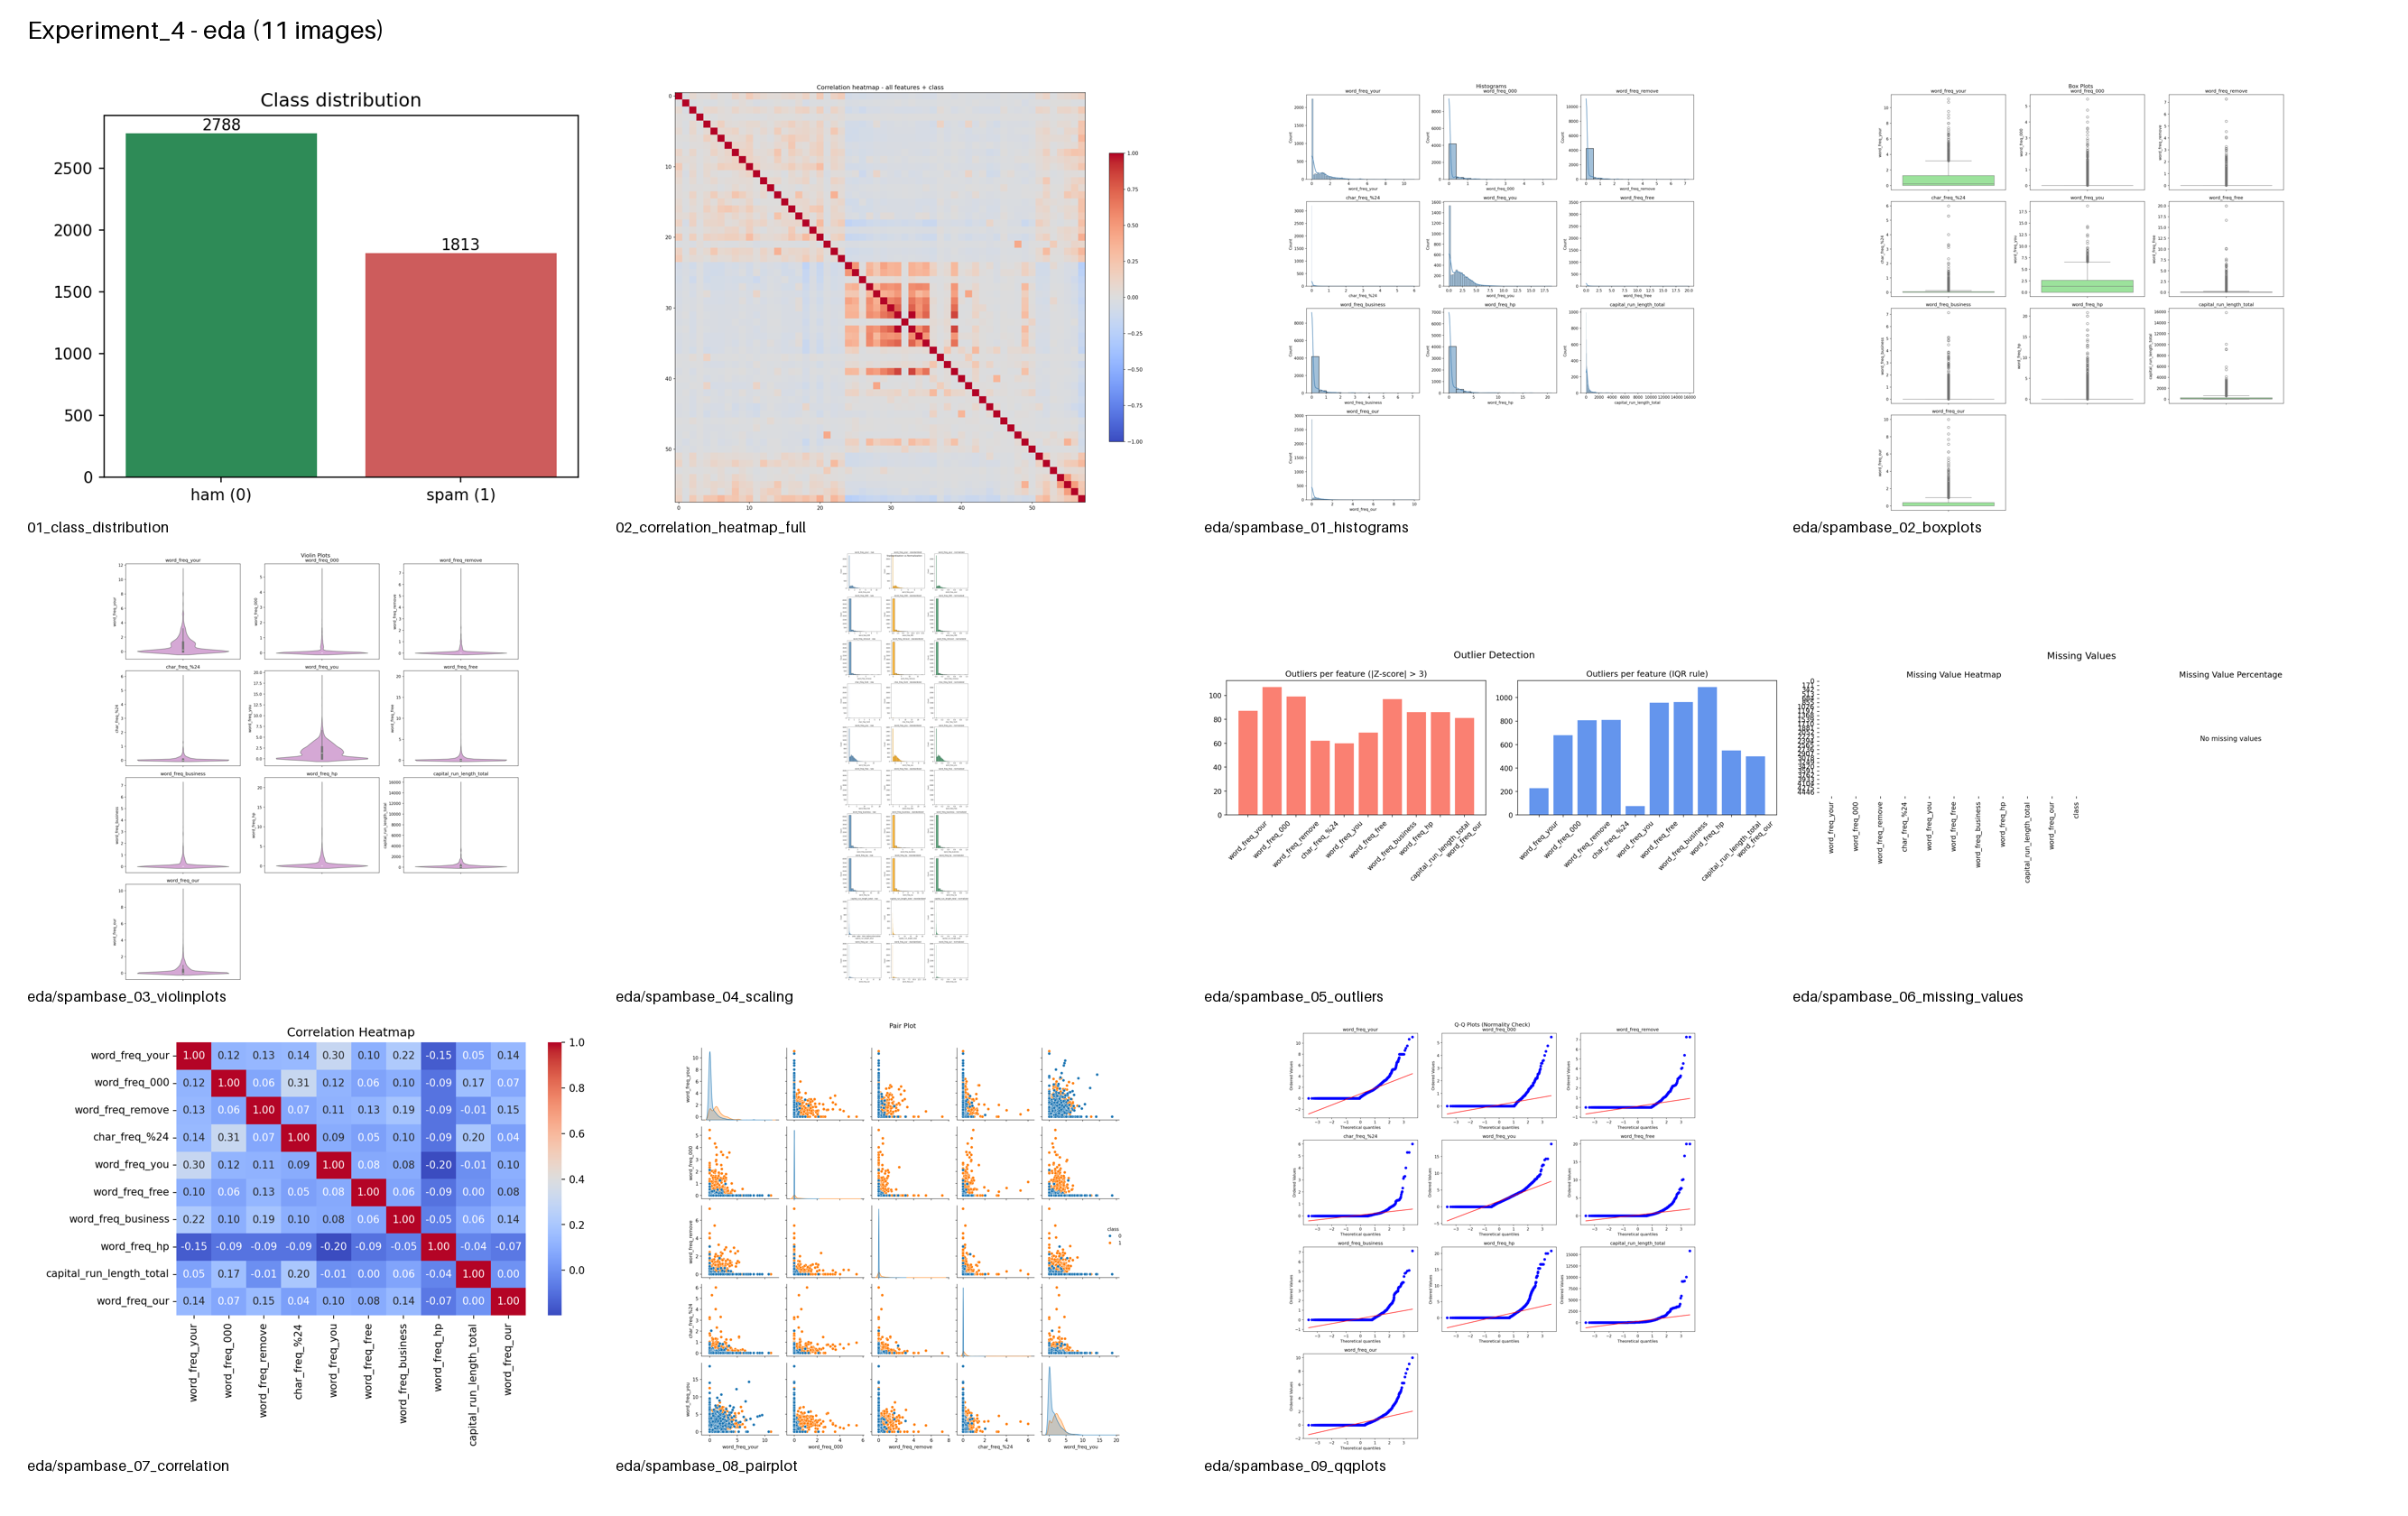
\includegraphics[width=0.95\linewidth]{outputs/Experiment_4_eda_combined.png}
\caption{Class distribution, full correlation heatmap, and histogram, box plot, violin, scaling,
outlier, pair plot and Q-Q panels for the ten most predictive features.}
\end{figure}

\textbf{Inference:}

Since this is the same underlying dataset as Experiment 2, the same features (word\_freq\_your,
word\_freq\_000, the exclamation and dollar sign frequencies) come out as the strongest spam
indicators again. What matters more for this particular experiment is the pair plot, the spam and ham
clusters overlap rather than sitting in neatly separated regions, which is an early hint that a linear
boundary might already be doing most of the heavy lifting.

\section{Data Preprocessing}
\begin{itemize}
\item No missing values, all features numeric already, no encoding needed.
\item StandardScaler applied before both Logistic Regression and SVM.
\item 80/20 stratified split, checked further with 5 fold cross validation.
\end{itemize}

\begin{lstlisting}[caption={Grid search for Logistic Regression and SVM across four kernels}]
lr_grid = GridSearchCV(LogisticRegression(max_iter=5000),
                        lr_param_grid, cv=5, scoring="accuracy")
lr_grid.fit(X_train_scaled, y_train)

svm_param_grid = [
    {"kernel": ["linear"], "C": [0.1, 1, 10]},
    {"kernel": ["rbf"], "C": [0.1, 1, 10], "gamma": ["scale", "auto"]},
    {"kernel": ["poly"], "C": [0.1, 1, 10], "degree": [2, 3]},
]
svm_grid = GridSearchCV(SVC(), svm_param_grid, cv=5, scoring="accuracy")
svm_grid.fit(X_train_scaled, y_train)
\end{lstlisting}

\section{Machine Learning Algorithm}

\textbf{Logistic Regression} models $P(y=1\mid x) = \dfrac{1}{1+e^{-(w^Tx+b)}}$, trained by minimizing
log loss. $C$ controls how strong the regularization is, a small $C$ keeps the boundary simple.

\textbf{Support Vector Machine} finds the hyperplane that maximizes the margin between classes, and
only the closest support vectors actually matter for where that boundary sits. The kernel trick lets
it draw non-linear boundaries without much extra cost, linear stays flat, RBF and polynomial curve,
and sigmoid behaves a bit like a single layer neural network. $C$ trades margin width against
misclassification, and $\gamma$ controls how far a single point's influence reaches.

\section{Experimental Setup}
\begin{tabular}{ll}
\toprule
Python Version & 3.11.9 \\
Scikit-Learn Version & 1.7.2 \\
IDE & Anaconda Navigator / VS Code \\
Operating System & Windows 11 \\
Hardware & \\
\bottomrule
\end{tabular}

\section{Hyperparameter Selection}
\begin{tabular}{ll}
\toprule
Parameter & Value\\
\midrule
LR grid & penalty L1/L2, C in \{0.01,0.1,1,10,100\}, solver liblinear/saga \\
SVM grid & kernel in \{linear,poly,rbf,sigmoid\}, C in \{0.1,1,10\}, gamma, degree(poly) \\
\bottomrule
\end{tabular}

\vspace{0.3cm}
\begin{tabular}{p{3.2cm}p{2.4cm}p{5.6cm}p{2.5cm}}
\toprule
Model & Search Method & Best Parameters & Best CV Accuracy \\
\midrule
Logistic Regression & Grid Search & C=1, penalty=L2, solver=saga & 0.9242 \\
SVM & Grid Search & C=10, gamma=scale, kernel=rbf & 0.9332 \\
\bottomrule
\end{tabular}

\section{Results}

\begin{tabular}{lc}
\toprule
Logistic Regression Metric & Value \\
\midrule
Accuracy & 0.9305 \\
Precision & 0.9211 \\
Recall & 0.9008 \\
F1 Score & 0.9109 \\
\bottomrule
\end{tabular}

\vspace{0.3cm}
\textbf{SVM Kernel-wise Performance}

\begin{tabular}{lccc}
\toprule
Kernel & Accuracy & F1 Score & Training Time (s) \\
\midrule
Linear & 0.9273 & 0.9063 & 11.98 \\
RBF & 0.9207 & 0.8976 & 1.52 \\
Sigmoid & 0.8893 & 0.8534 & 2.14 \\
Poly & 0.9164 & 0.8902 & 1.68 \\
\bottomrule
\end{tabular}

\vspace{0.3cm}
\textbf{Comparative Analysis}

\begin{tabular}{lcc}
\toprule
Criterion & Logistic Regression & SVM \\
\midrule
Accuracy & 0.9305 & 0.9273 \\
Model Complexity & Low & High \\
Training Time & Low & High \\
Interpretability & High & Low \\
\bottomrule
\end{tabular}

\section{Result Visualization}

\begin{figure}[H]
\centering
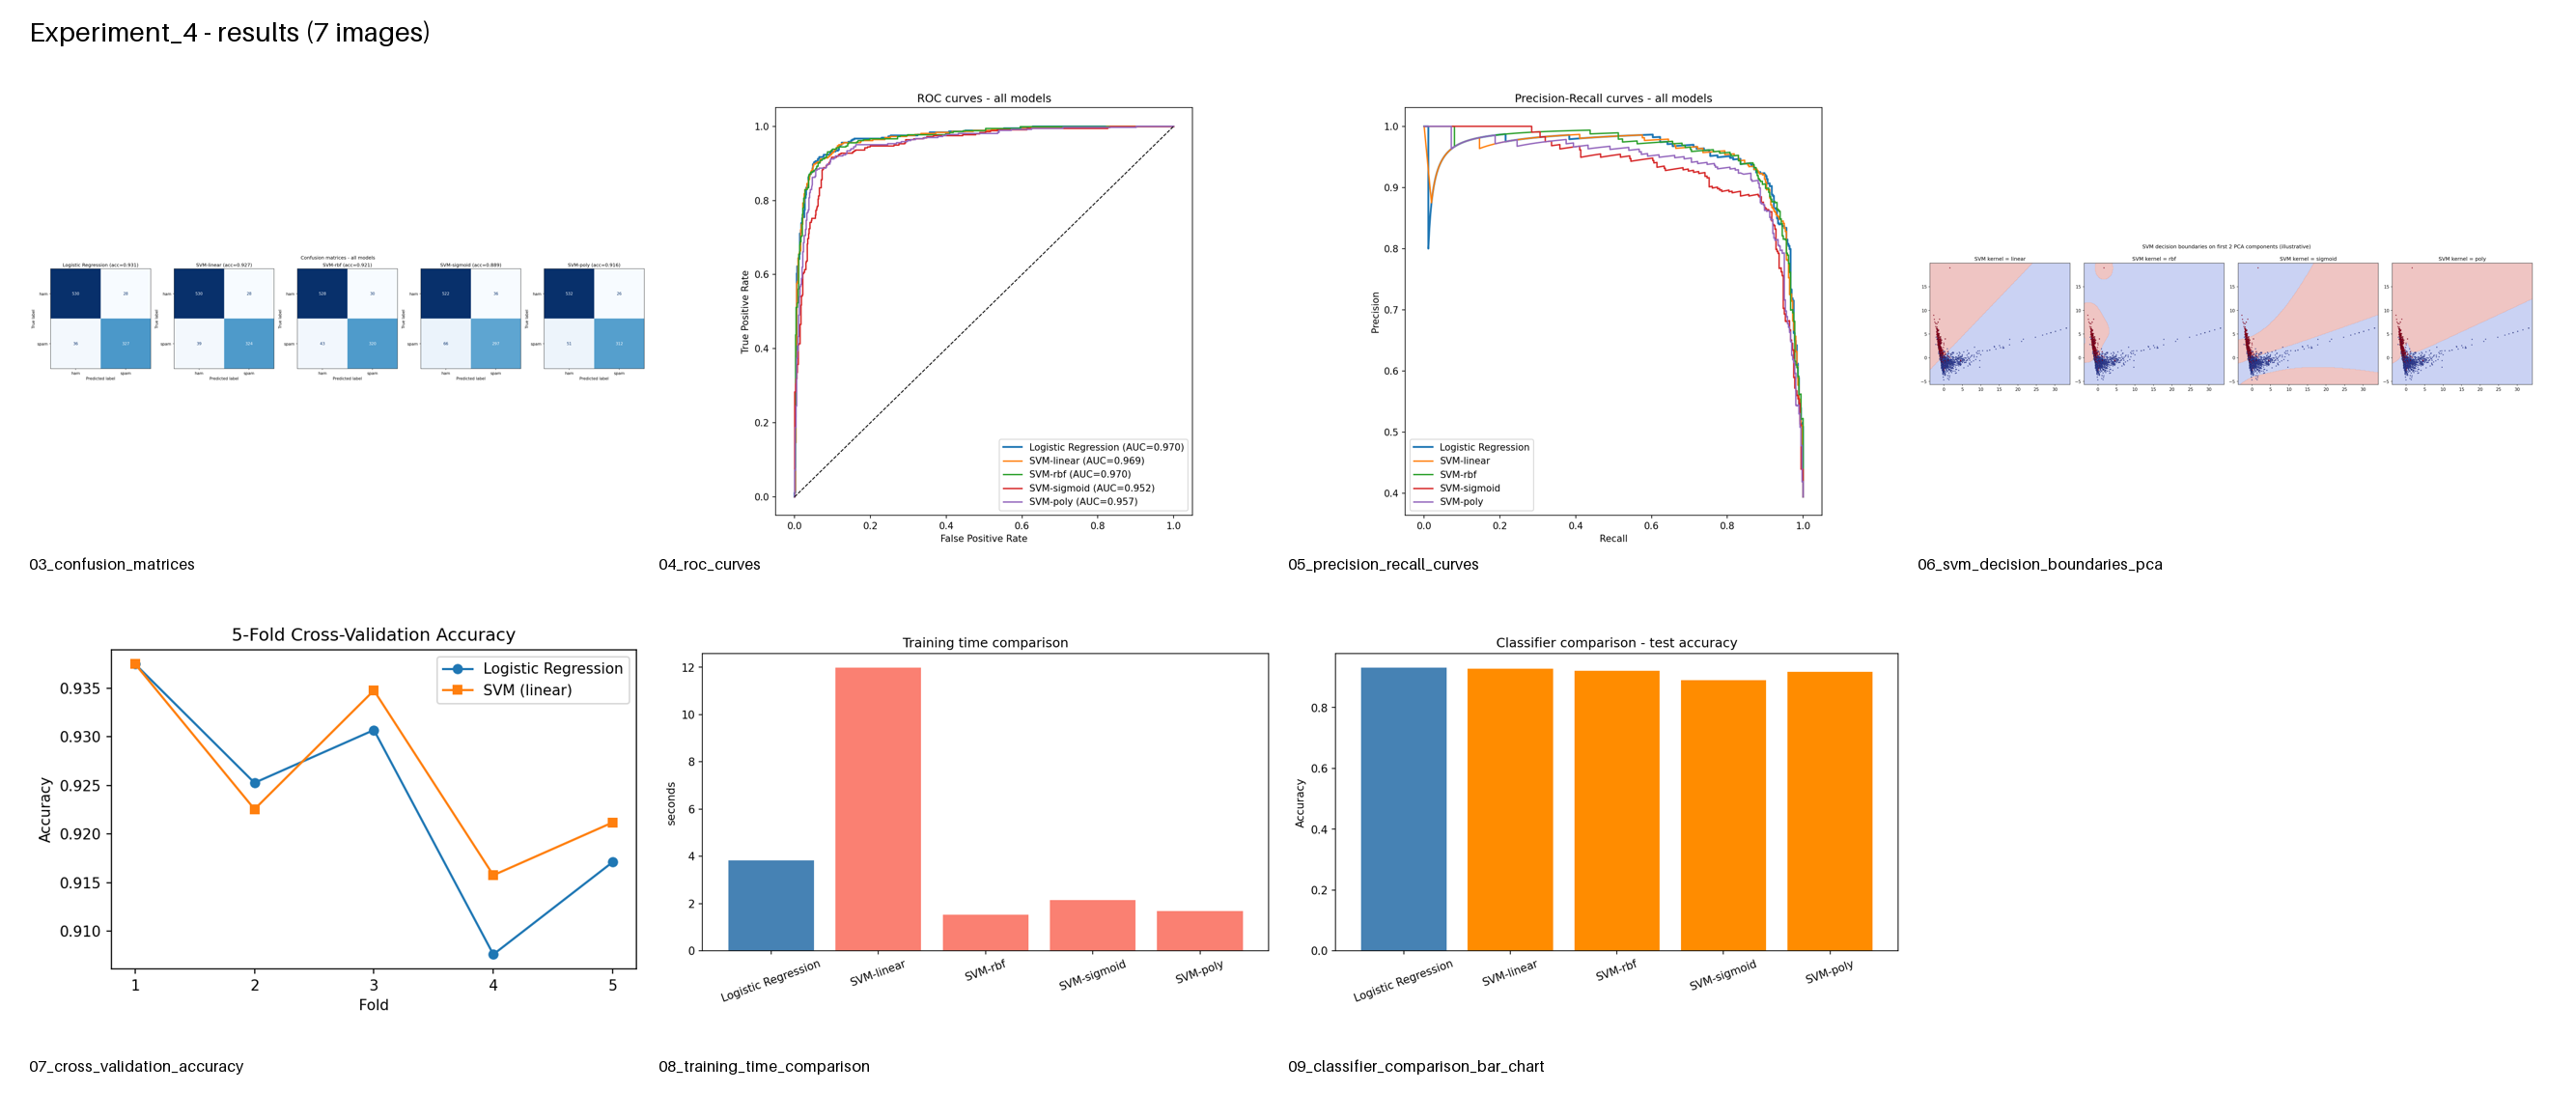
\includegraphics[width=0.95\linewidth]{outputs/Experiment_4_results_combined.png}
\caption{Confusion matrices and ROC/precision-recall curves for Logistic Regression and all four SVM
kernels, SVM decision boundaries on the first two PCA components, cross validation accuracy, and
training time and accuracy comparison bars.}
\end{figure}

\textbf{Inference:}

Logistic Regression and linear SVM produce almost identical confusion matrices, which is a pretty
strong sign the real boundary here is close to linear to begin with. The PCA decision boundary plot
backs this up nicely, linear and RBF carve up the space in very similar ways while sigmoid looks
noticeably messier, matching sigmoid landing dead last on accuracy at 0.8893. Training time gave the
most lopsided chart of the bunch, linear SVM takes around 12 seconds against just 1.5 to 2 seconds for
the other kernels, probably because Spambase is not perfectly linearly separable, so the solver has to
work harder to find a margin that still keeps mistakes low.

\section{Discussion}
Logistic Regression comes out ahead on nearly every axis that matters, slightly higher test accuracy
(0.9305 versus SVM's best of 0.9273), much faster training, and coefficients you can actually inspect
afterward. RBF does edge it out a little on CV accuracy (0.9332 versus 0.9242), so the two are genuinely
close, but that small edge does not really seem worth the extra training cost and lost interpretability
for something like spam filtering, where knowing which features triggered a flag actually matters.
Sigmoid's weak showing lines up with its usual reputation of only really working in a narrow band of
parameters.

\section{Conclusion}
For Spambase specifically, Logistic Regression matches or slightly beats every SVM kernel while
training far faster and staying easy to interpret, which makes it the practical pick here. RBF SVM
stays a reasonable backup option if a bigger or higher dimensional dataset ever introduced more real
non-linear structure to exploit.

\section{Learning Outcomes}
\begin{itemize}
\item Confirmed that a kernel method is not automatically the better choice, on data that is already
close to linearly separable, the extra flexibility barely helps and just costs real training time.
\item Got practice reading a PCA projected decision boundary as a quick sanity check for why one kernel
is beating another.
\item Saw concretely how $C$ and $\gamma$ actually reshape an SVM boundary, not just in theory but in
the accuracy numbers themselves.
\item Learned to weigh accuracy against interpretability and training cost when picking a model,
instead of just chasing whatever number is highest.
\end{itemize}

\section{References}
\begin{enumerate}
\item Stephen Marsland, ``Machine Learning - An Algorithmic Perspective'', 2nd Edition, Chapman and
Hall/CRC Machine Learning and Pattern Recognition Series, 2015.
\item Ethem Alpaydin, ``Introduction to Machine Learning'', 3rd Edition, The MIT Press, 2014.
\end{enumerate}

\end{document}
